\documentclass[a4paper]{exam}

\usepackage{amsmath,amsfonts}
\usepackage{geometry}
\usepackage{graphicx}
\usepackage{hyperref}
\usepackage{tabularx}

\printanswers

\title{Weekly Challenge 04: Divive-and-Conquer Convex Hull}
\author{User 1 \and User 2}  % replace with your GitHub user names
\date{CS 412 Algorithms: Design and Analysis\\Spring 2022}

\graphicspath{{images/}}

\begin{document}
\maketitle

\begin{questions}

  \begin{figure}[h]
    \begin{tabularx}{\textwidth}{cc}
    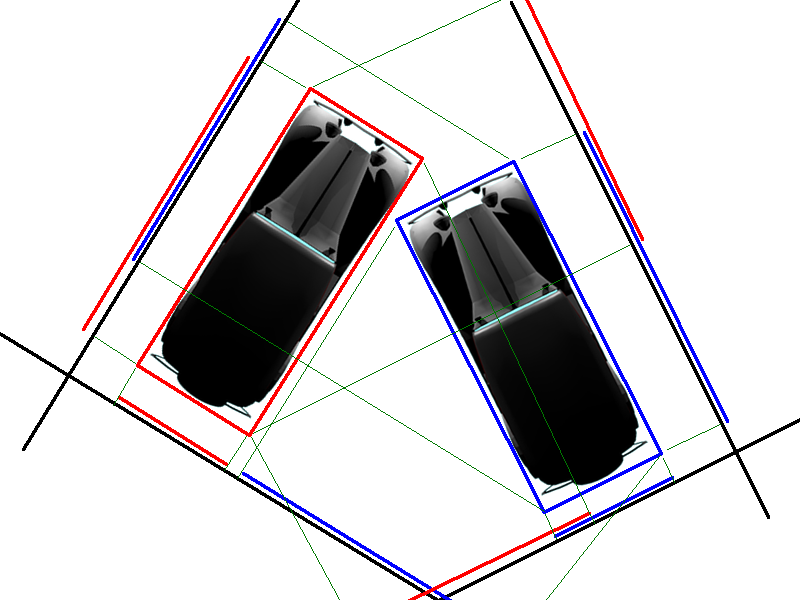
\includegraphics[width=.45\textwidth]{collisionDetect500}
      &
      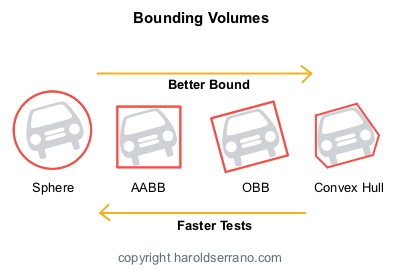
\includegraphics[width=.45\textwidth]{methods}\\
      \\
      (a) & (b)
    \end{tabularx}
    \caption{(a) Collision between cars \cite{collision}. (b) The accuracy and computation speed of different collision detection methods \cite{tips}.}
    \label{fig:methods}
  \end{figure}
  
\question \textit{Collision detection} is an important operation in many games. The \textit{convex hull} of a shape is defined as ``the smallest convex shape that fully contains it. For a concave polygon in two dimensions, it would be like hammering a nail on each vertex and wrapping a rubber band around all nails'' \cite{physics}. It is one of the more accurate methods to compute collisions \cite{tips}. The following diagram, taken from \cite{jarvis}, shows (a) $n$ points in a plane and (b) their convex hull.
  
  \centerline{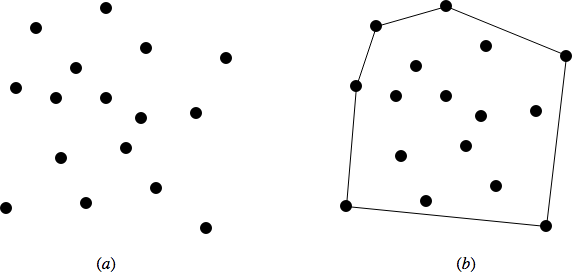
\includegraphics[width=.6\textwidth]{hull}}

  \textbf{TASKS}:
  \begin{parts}
  \part Generate $n$ random points in a plane and apply a divide-and-conquer algorithm to compute their convex hull.
  \part Visualize the $n$ points and key stages in the evolution of the solution as an animation, e.g. an animated GIF, in order to illustrate the working of your algorithm.
  \part Include below some of the key visualizations.
  \part Share your animation as a comment on the \textit{Week 04 Challenge} post in the course group on Yammer.
  \end{parts}
  
  \begin{solution}
    % Enter your solution here.
  \end{solution}


\end{questions}

\begin{thebibliography}{9}
\bibitem{collision}
  3D Theory - Example - Car Racing Game - collisions, \url{http://www.euclideanspace.com/threed/games/examples/cars/collisions/}, last accessed on 4 Feb 2022.

  \bibitem{tips}
Tips for developing a Collision Detection System, \url{https://www.haroldserrano.com/blog/tips-for-developing-a-collision-detection-system}, last accessed on 4 Feb 2022.

\bibitem{physics}
Video Game Physics Tutorial - Part II: Collision Detection for Solid Objects, \url{https://www.toptal.com/game/video-game-physics-part-ii-collision-detection-for-solid-objects}, last accessed on 4 Feb 2022.

\bibitem{jarvis}
Convex Hull Algorithms: Jarvis's March, \url{https://algorithmtutor.com/Computational-Geometry/Convex-Hull-Algorithms-Jarvis-s-March/}, last accessed on 4 Feb 2022.
\end{thebibliography}
\end{document}

%%% Local Variables:
%%% mode: latex
%%% TeX-master: t
%%% End:
